The primary result of this project is a dataset of synthetic images generated using Unity, highlighting the flexibility and capabilities of the Unity Perception package. The dataset, which includes over XXXX images of different boats and objects in a maritime environment, is designed to support machine learning tasks, particularly for scenarios where acquiring large-scale, annotated real-world data is difficult. By leveraging Unity's randomization features, the dataset encompasses a variety of scenarios, including different lighting conditions and weather effects, making it well-suited for applications in boat docking and other maritime tasks.

\section{Images}
 These images generated show the potential of synthetic data in machine learning tasks, particularly for scenarios where acquiring large-scale, annotated real-world data is challenging. The generated dataset combines diverse and labeled images with a focus on maritime environments, making it well-suited for applications in this domain. The images generated is a dataset with over xxxx images of different boats and object in the sea. 
\begin{table}[H]
\centering
\begin{tabular}{|l|c|c|}
\hline
\multicolumn{3}{|c|}{\textbf{Dataset Distrobution}} \\ 
\hline
\textbf{Object Type} & \textbf{Total Images} & \textbf{Rainy Images} \\ 
\hline
Boat         & 1,000  & 20  \\ 
Sailboat     & 300    & 20  \\ 
Kayak        & 100    & 50  \\ 
Buoy         & 200    & 50  \\ 
Windsurfer   & 200    & 50  \\ 
\hline
\textbf{Total}       & \textbf{1,800} & \textbf{190} \\ 
\hline
\end{tabular}
\caption{Breakdown of the dataset by object type and weather condition.}
\label{tab:dataset_composition}
\end{table}



\begin{figure}[H]
\centering
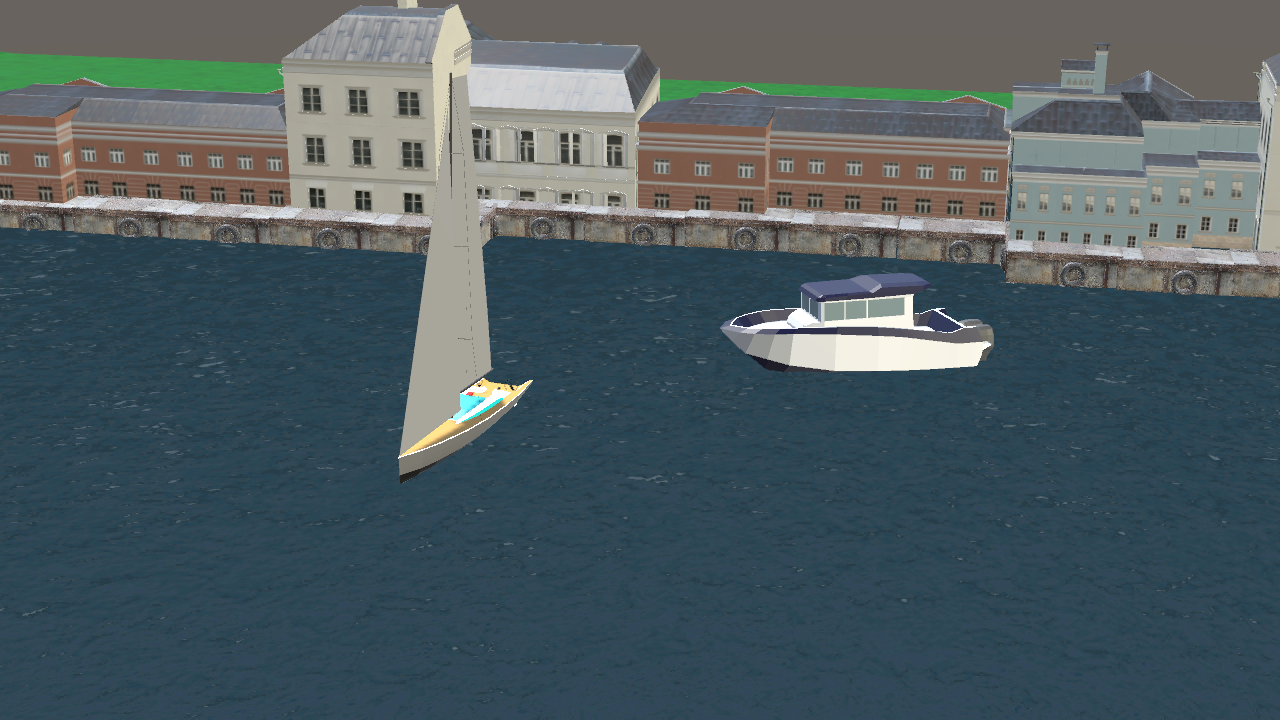
\includegraphics[width=0.7\textwidth]{Figures/rgb_2.png}
\caption{Example of one of the images in the dataset}
\label{fig:original_image}
\end{figure}

\section{Dataset Diversity}
A key goal of this project was to ensure that the dataset reflects a wide variety of scenarios, including different lighting conditions, object arrangements, and environmental setups. Using Unity's Perception package, randomization techniques were applied to introduce significant variability across the dataset. This included adjustments to object rotations, positions, and textures, as well as environmental factors like lighting angles and weather.

\subsection{Randomization}
The Perception package offers a set of randomizers that were instrumental in enhancing the diversity. Randomization helps generate datasets that are more generalizable, reducing the risk of overfitting models trained on synthetic data. Below are examples of randomized images showcasing different configurations of the maritime environment.

\begin{figure}[H]
\centering
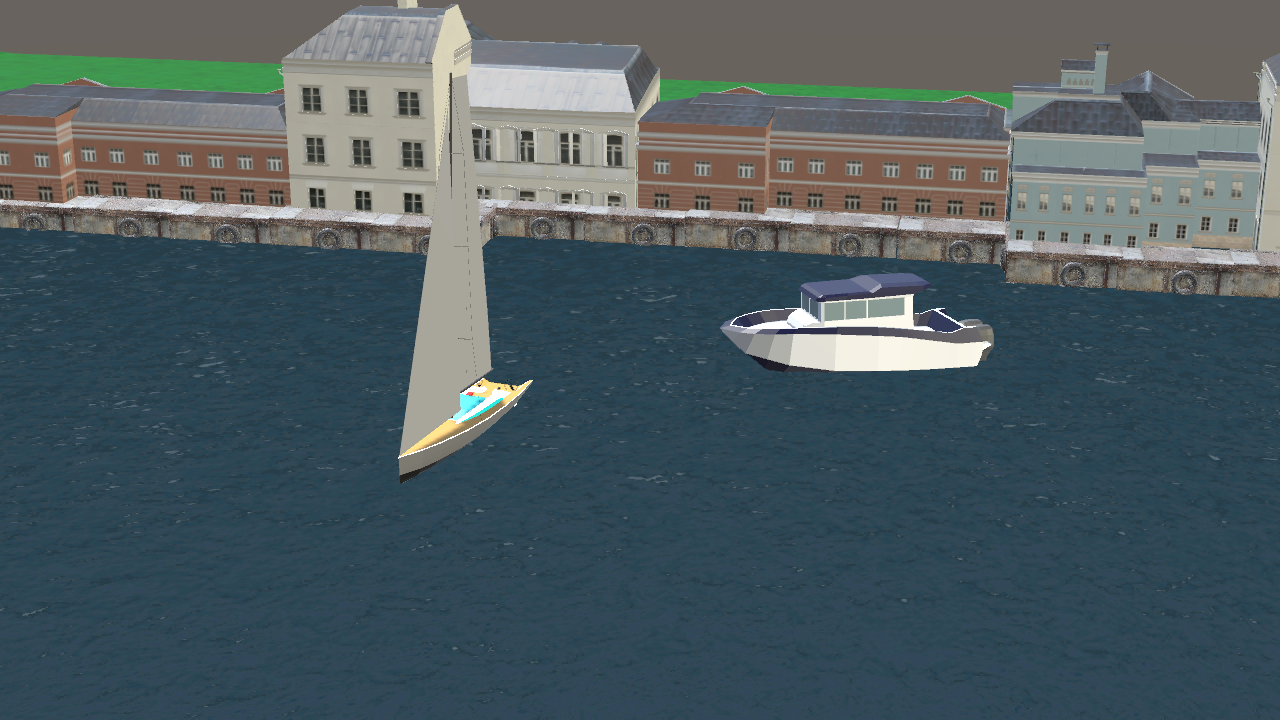
\includegraphics[width=0.32\textwidth]{Figures/rgb_2.png}
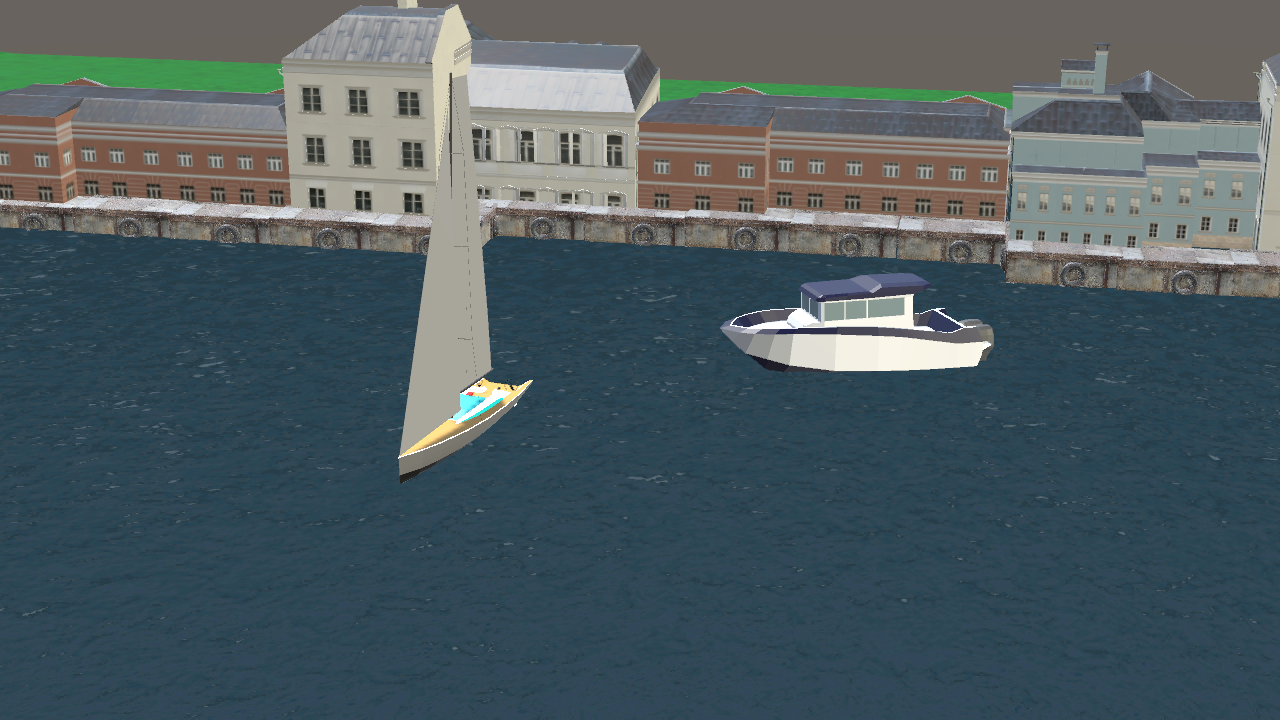
\includegraphics[width=0.32\textwidth]{Figures/rgb_2.png}
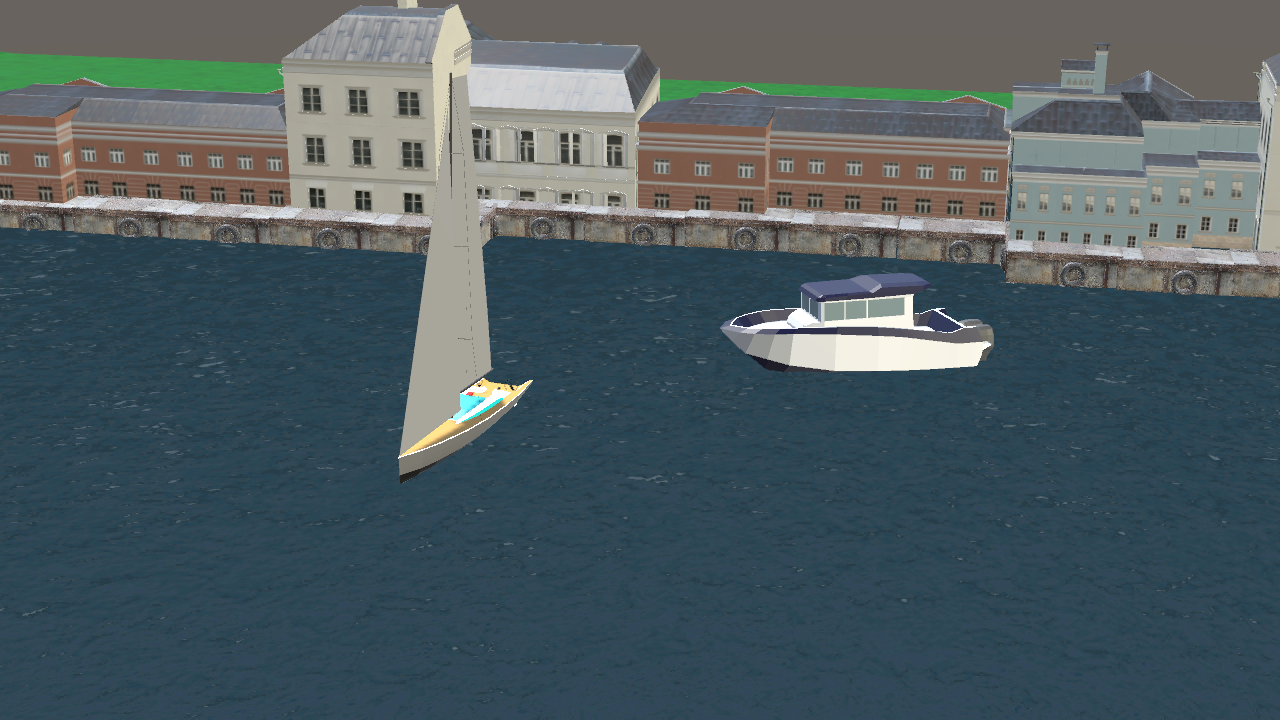
\includegraphics[width=0.32\textwidth]{Figures/rgb_2.png}
\caption{Example of 3 randomized images with the same target.}
\label{fig:randomized_images}
\end{figure}

\section{Labeling}
Another important feature of the Unity Perception package is the ability to automatically generate labels for synthetic images, including segmentation masks and bounding boxes. This automation significantly reduces the manual effort required for labeling while ensuring high accuracy and consistency. Below is an example comparing an original image with its segmentation-label, showing the precision of the labeling process.

\begin{figure}[H]
\centering
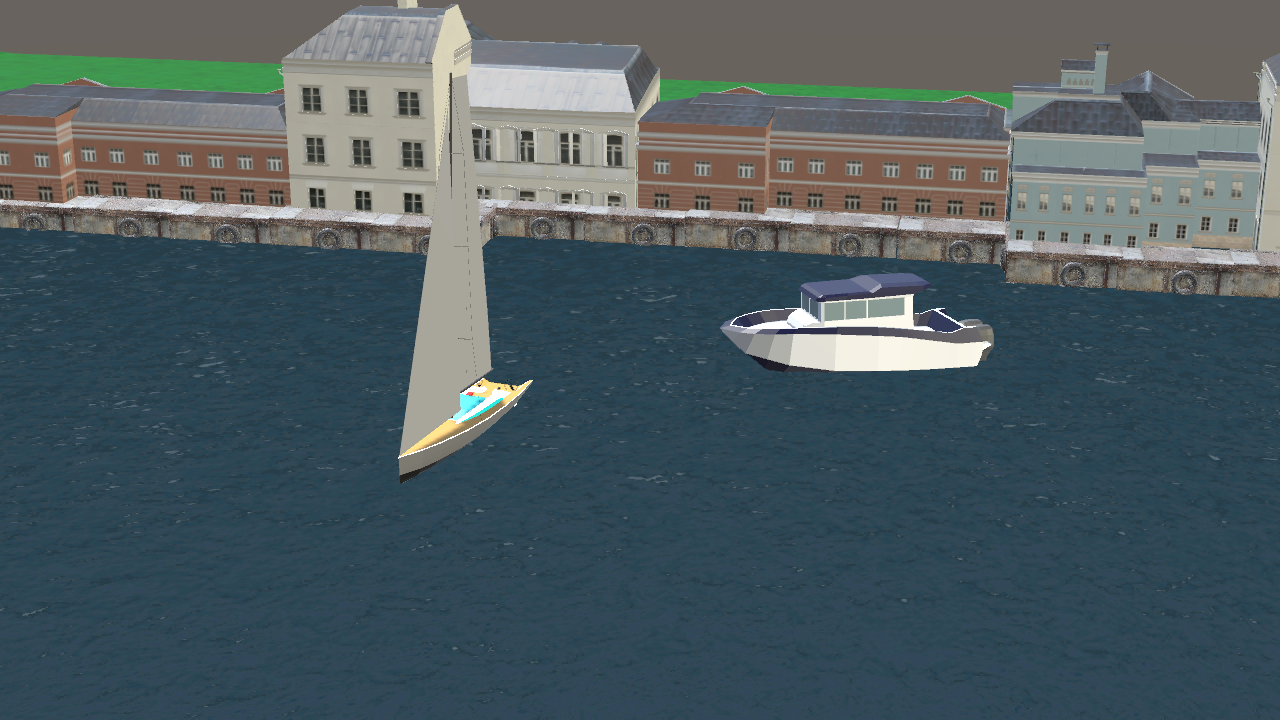
\includegraphics[width=0.49\textwidth]{Figures/rgb_2.png}
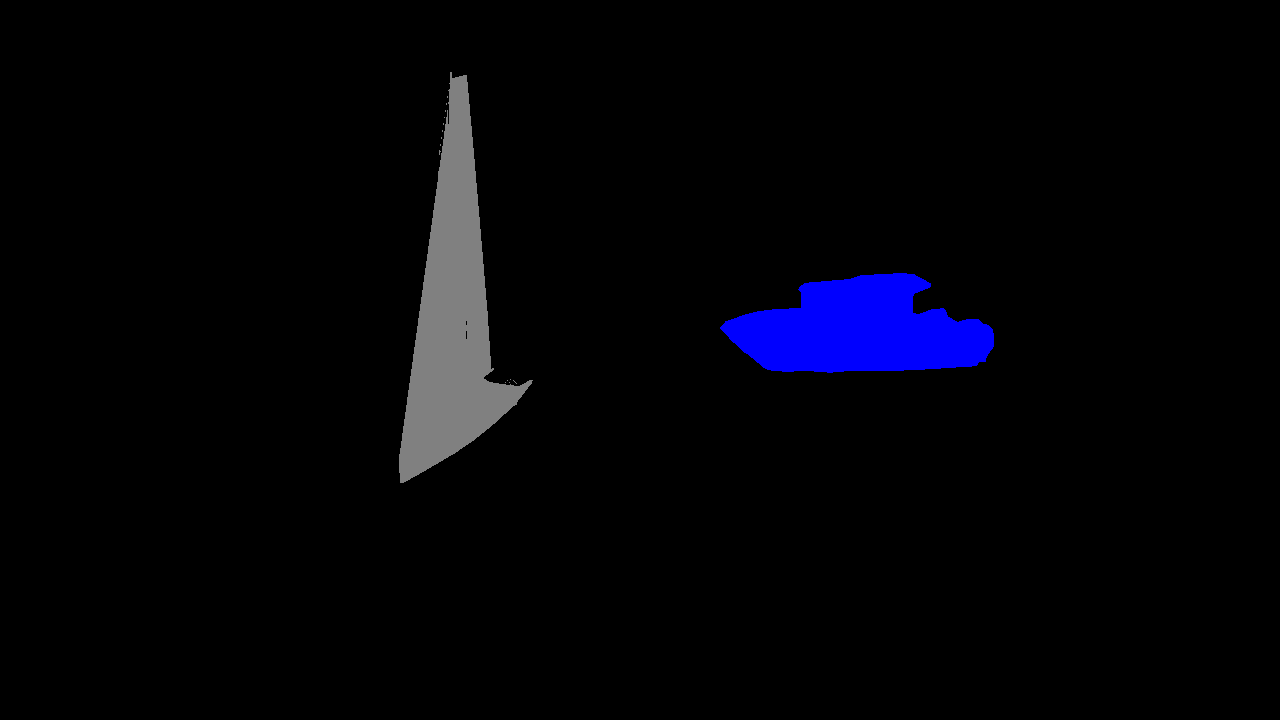
\includegraphics[width=0.49\textwidth]{Figures/segmentation_2.png}
\caption{Comparison of the original image and its labeled segmentation output.}
\label{fig:labeled_images}
\end{figure}

\section{Discussion}
\subsection{Performance of the 3D Models and Environment}
The generated images are visually compelling but limited by the quality of free assets used in the project. While the water simulation adds a layer of dynamism and realism, other environmental elements like docks and boats relied on low-poly models. This limitation impacted the overall fidelity of the scenes, which may reduce their suitability for certain machine learning tasks requiring high levels of detail or photorealism.

\subsection{Challenges and Limitations}
Several challenges arose during the project, particularly related to Unity's version compatibility and asset rendering. In some cases, imported materials were incompatible with the project's Unity version, resulting in objects turning pink or failing to render. These issues were especially problematic for water simulations, limiting the variety of usable assets and scenes.\\

\noindent Additionally, the reliance on free or low-cost assets restricted the overall visual fidelity of the generated images. Future projects could benefit from investment in high-quality assets or collaborations with designers to create custom 3D models tailored to specific needs.

\subsection{Comparison to Real-World Data}
While synthetic datasets generated using Unity offer significant advantages in terms of scalability and labeling automation, they still face challenges in matching the realism and complexity of real-world data. The inclusion of randomization and AI-enhanced images bridges this gap to some extent, but further improvements are needed to fully replicate the intricacies of natural environments.

\subsection{Using AI to Enhance Results}
To address the limitations of asset quality, AI-based tools such as Stable Diffusion, accessed via the Dezgo platform, can be employed to enhance the visual quality of the Unity-generated images. These tools added a layer of photorealism, making the dataset more visually appealing and potentially more effective for training models. The example below illustrates the transformation achieved through AI-based enhancement.
\begin{figure}[H]
\centering
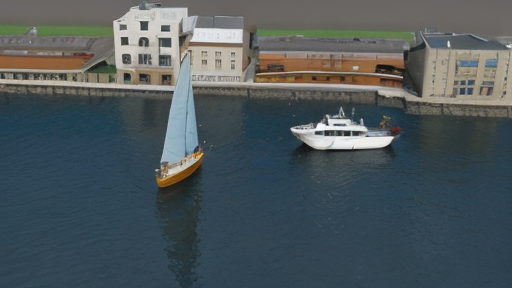
\includegraphics[width=0.49\textwidth]{Figures/photorealistic_3613113118.png}
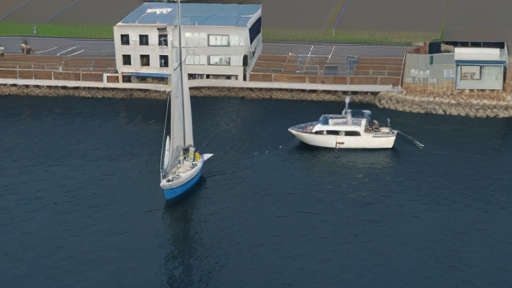
\includegraphics[width=0.49\textwidth]{Figures/photorealistic_2942539231.png}
\caption{AI-enhanced images generated using Dezgo.}
\label{fig:ai_enhanced}
\end{figure}

This combination of Unity-generated images and AI-driven post-processing opens new possibilities for creating high-quality synthetic datasets with minimal additional effort, which is worth checking out for next semester.
